\documentclass{beamer}

\usetheme{cern}

\author{Dylan Gilbert}
\title{Monte Carlo vs Data Driven Estimates in $M_{T2}$}
\date{Mon June 12}

\begin{document}

\begin{frame}
\titlepage
\end{frame}

\begin{frame}{$Z->\nu\nu$ SR 1VL}
\begin{columns}
\begin{column}{0.3\textwidth}
\begin{flushleft}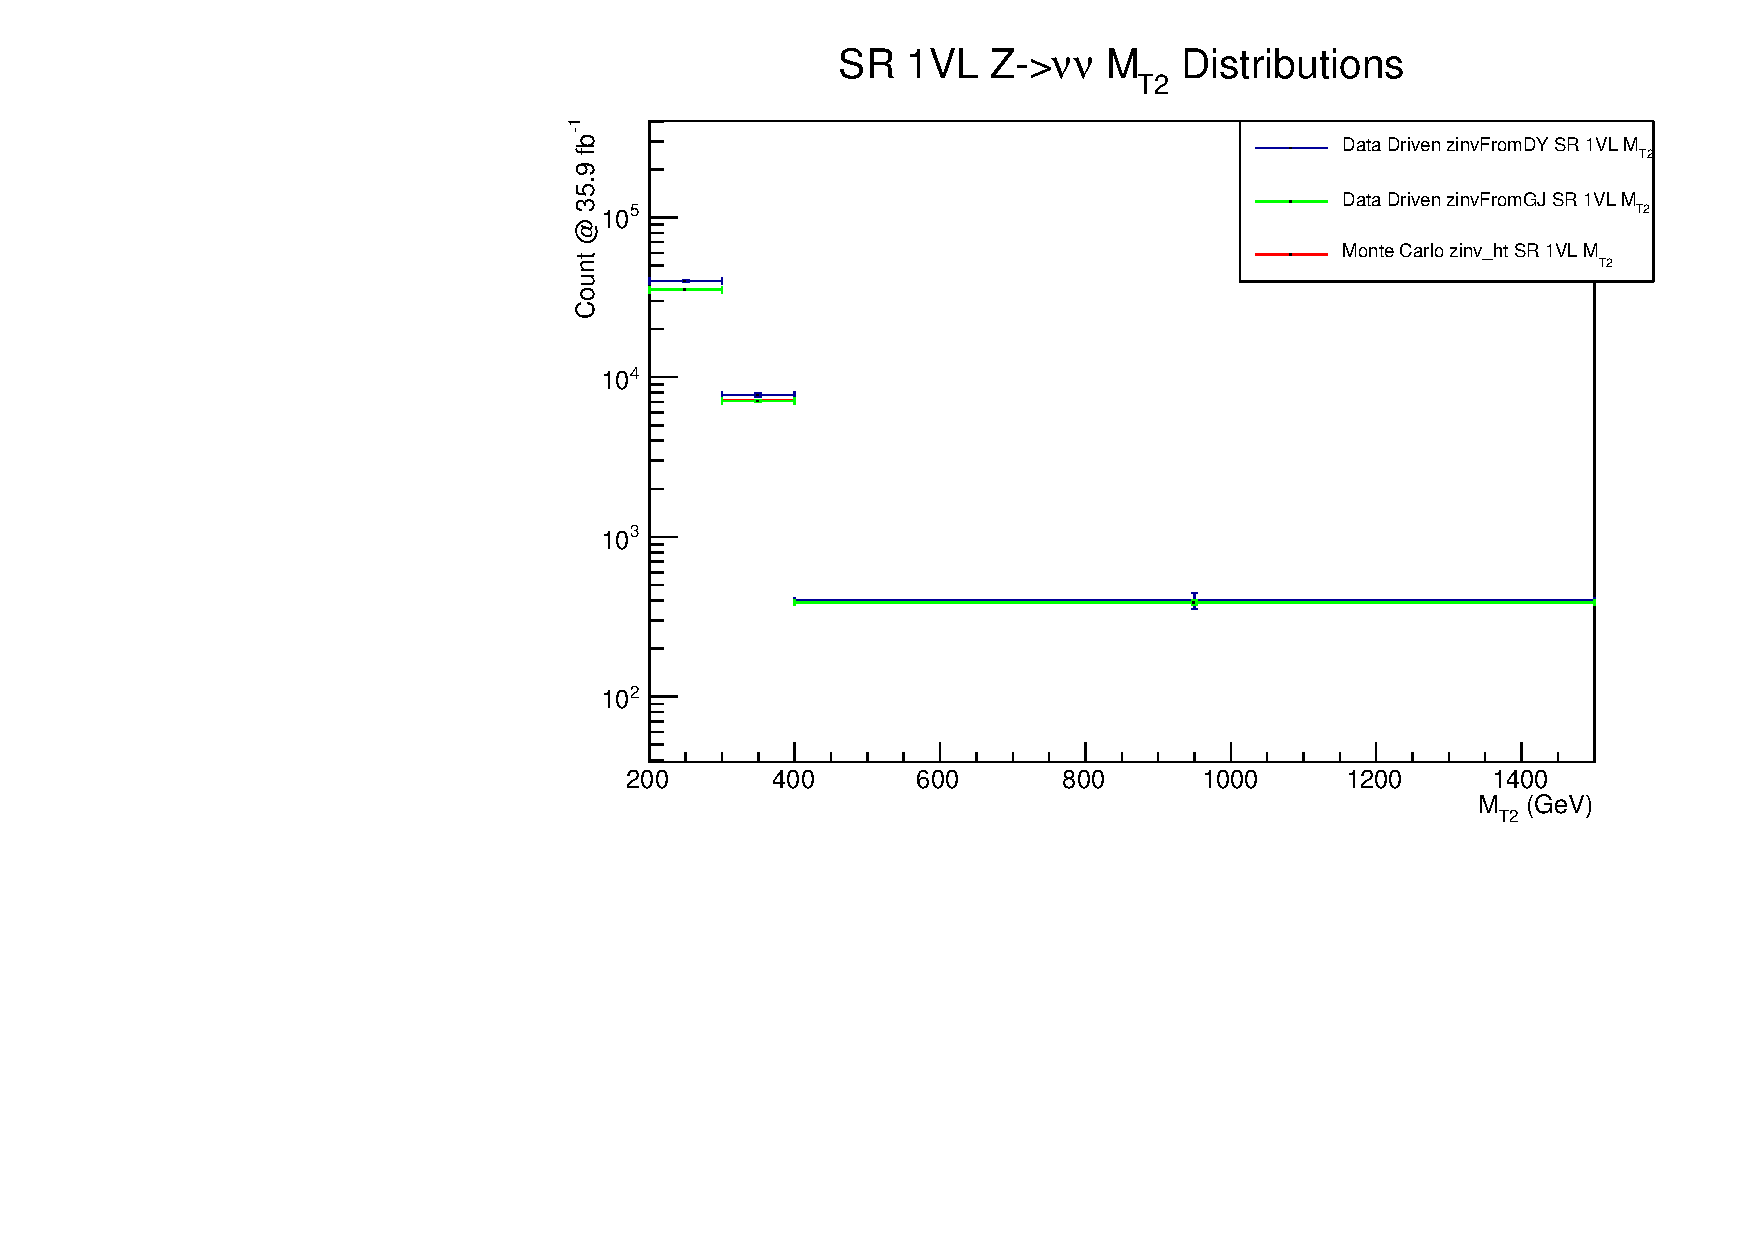
\includegraphics[scale=0.2]{PDFs/zinv_estimates_1VL}\end{flushleft}
\end{column}
\begin{column}{0.3\textwidth}
\begin{center}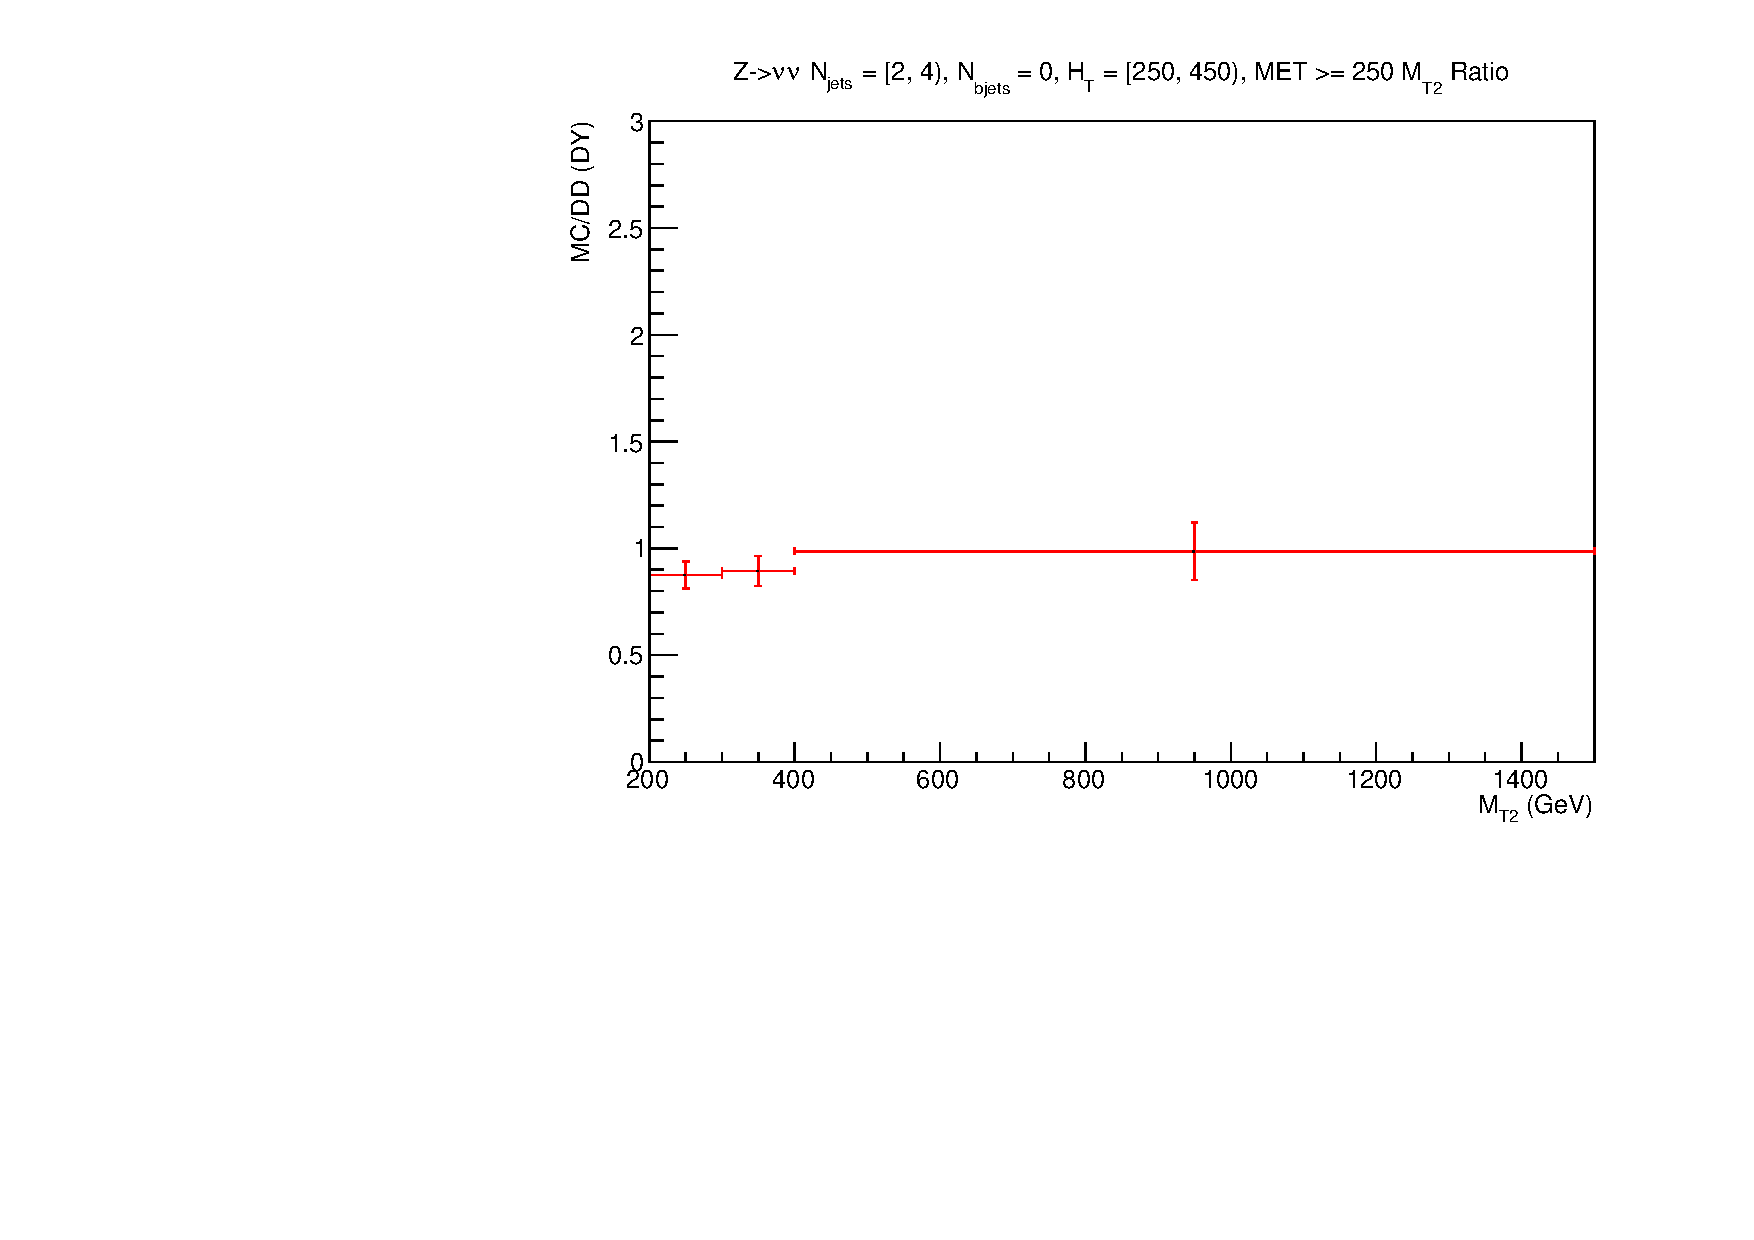
\includegraphics[scale=0.2]{PDFs/zinv_ratio_dy_1VL}\end{center}
\end{column}
\begin{column}{0.3\textwidth}
\begin{flushright}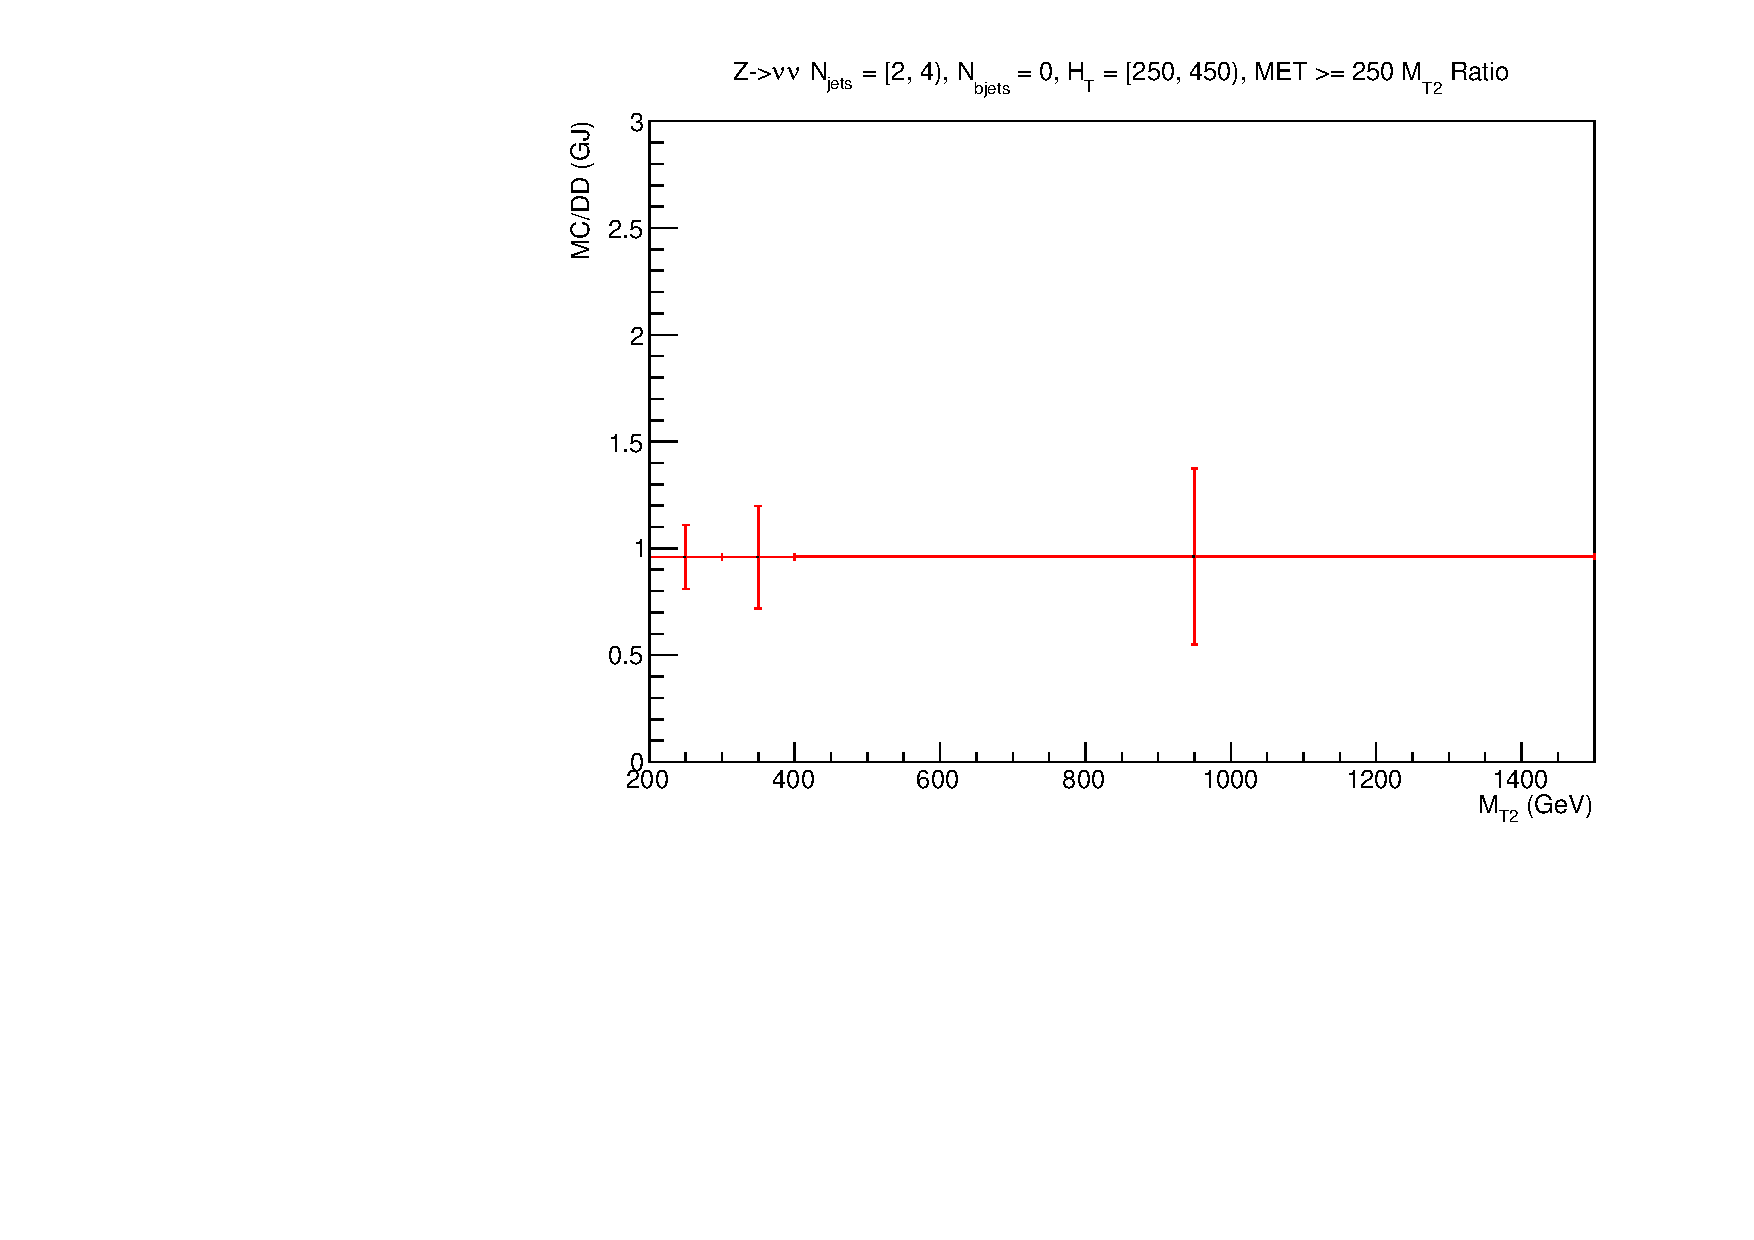
\includegraphics[scale=0.2]{PDFs/zinv_ratio_gj_1VL}\end{flushright}
\end{column}
\end{columns}
\begin{itemize}
\item MC and DD are similar, especially for $\gamma$.
\item Yes, MC is in the left plot, but overlaps with $\gamma$.
\item In high statistics bins, MC is robust for electroweak physics.
\end{itemize}
\end{frame}

\begin{frame}{Lost Lepton SR 1VL}
\begin{columns}
\begin{column}{0.5\textwidth}
\begin{flushleft}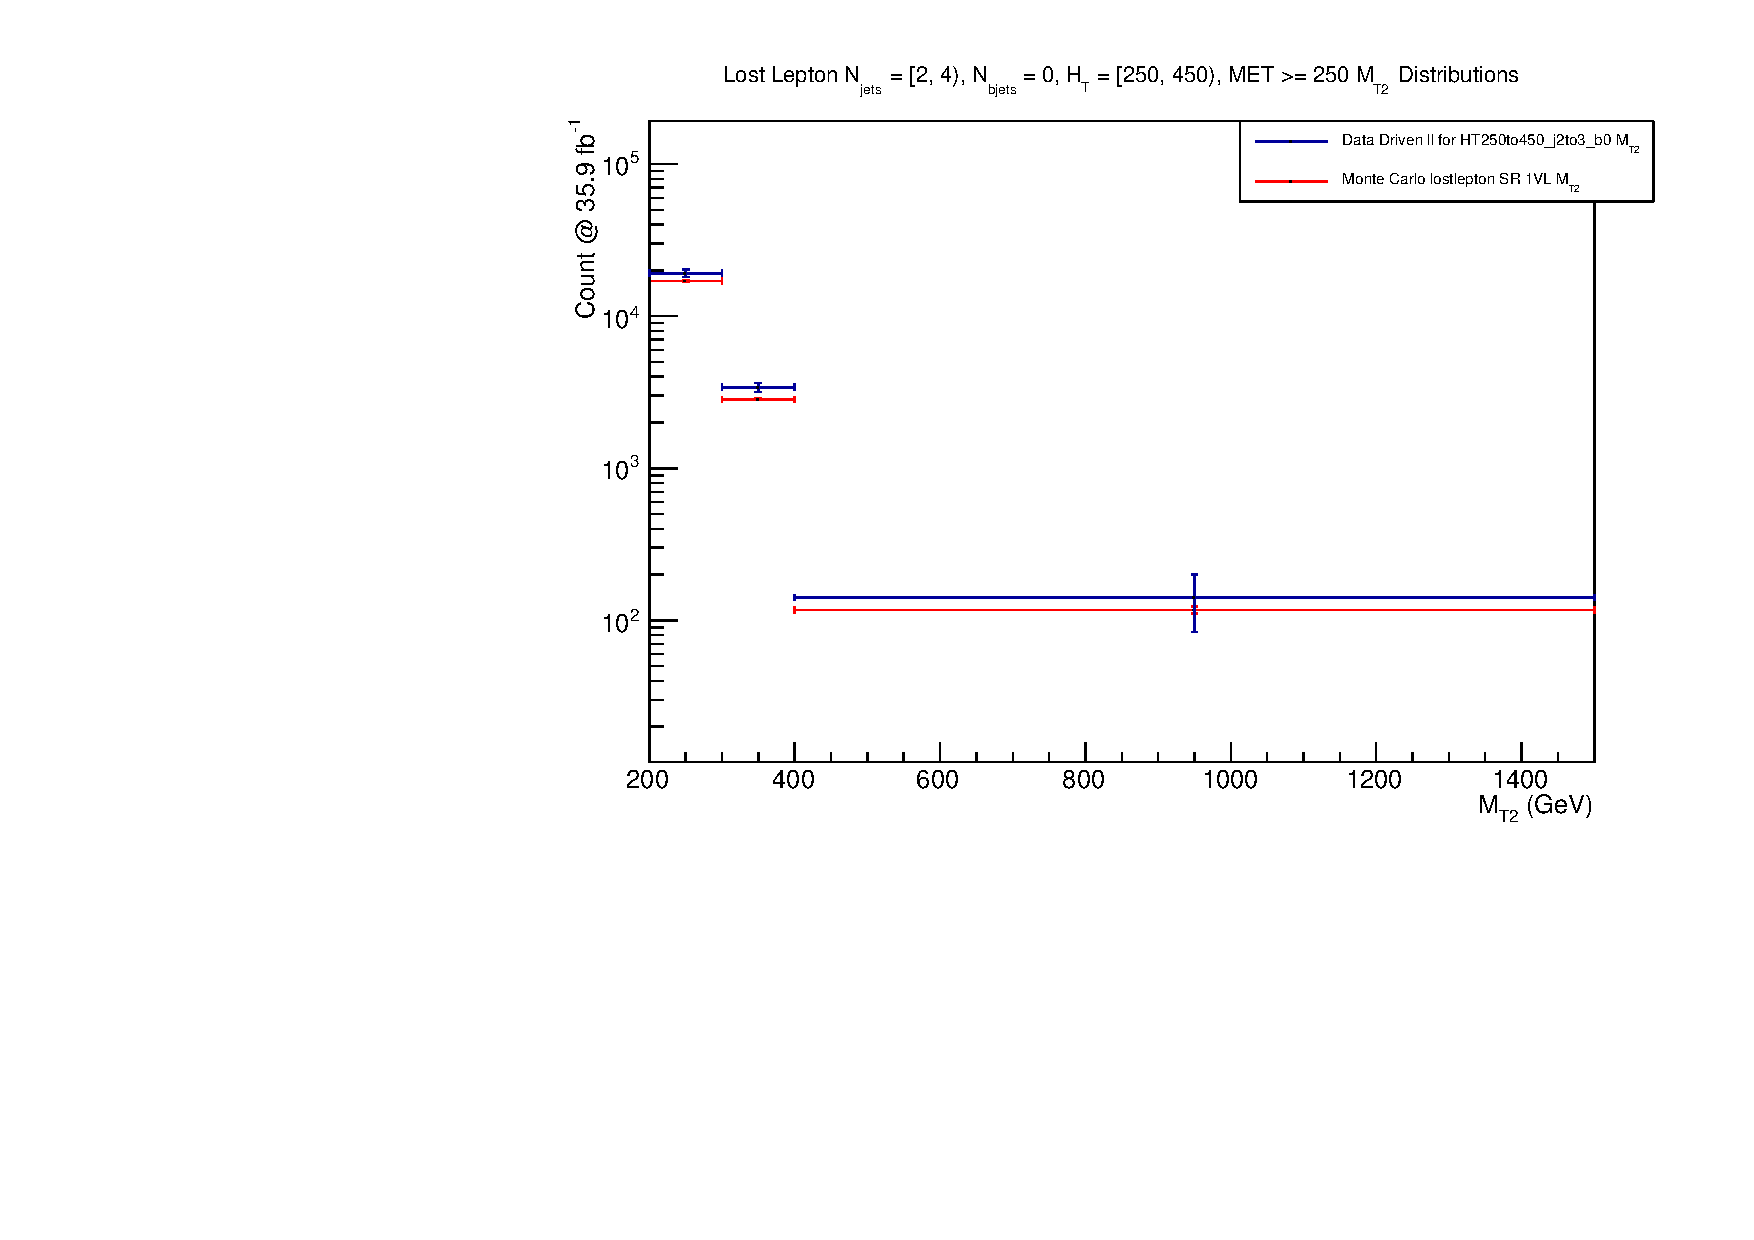
\includegraphics[scale=0.3]{PDFs/lostlep_estimates_1VL}\end{flushleft}
\end{column}
\begin{column}{0.5\textwidth}
\begin{flushright}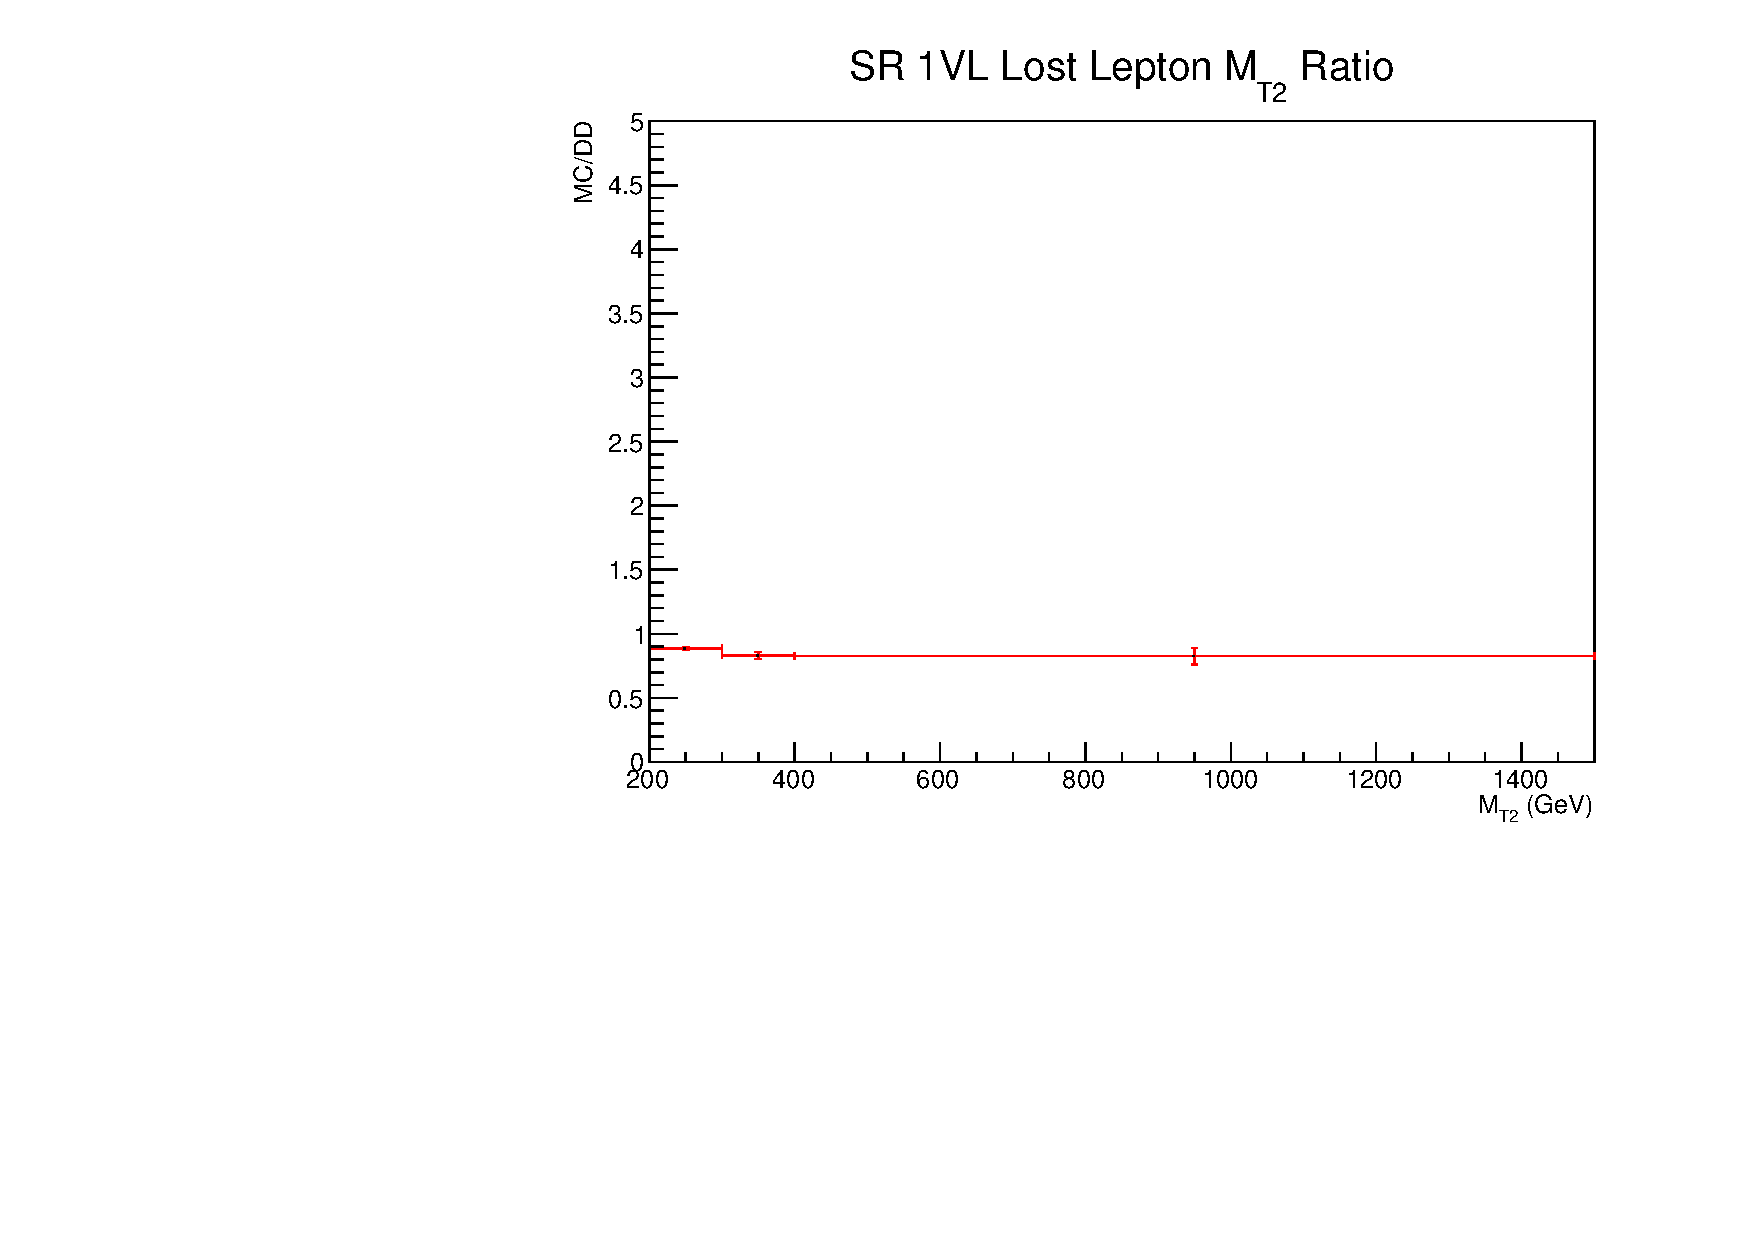
\includegraphics[scale=0.3]{PDFs/lostlep_ratio_1VL}\end{flushright}
\end{column}
\end{columns}
\begin{itemize}
\item MC fairly accurate but consistently underestimates.
\end{itemize}
\end{frame}

\end{document}
